% Some help here: https://en.wikibooks.org/wiki/LaTeX/Document_Structure

% Preamble
% ---
\documentclass{report}

% Packages
% ---
\usepackage{graphicx} % Add pictures to your document
\graphicspath{ {images/} }  % we will keep our images ogranized under the images directory
\usepackage{listings} % Source code formatting and highlighting
\usepackage{xcolor}   % needed to color hyperlinks and source code
\usepackage{hyperref} % create hyperlinks
\usepackage[T1]{fontenc} % make sure quotes in Python listings are straight quotes
\usepackage{tcolorbox}
\usepackage{siunitx} % Allows us to use math symbols (like Omega) in normal paragraphs

\hypersetup{
    colorlinks=true, %set true if you want colored links
    linktoc=all,     %set to all if you want both sections and subsections linked
    linkcolor=blue,  %choose some color if you want links to stand out
}

\lstloadlanguages{Python}
\lstset{
  language=Python,
  numberstyle=\color{gray},
  stringstyle=\color[HTML]{933797},
  commentstyle=\color[HTML]{228B22},
  emph={[2]from,import,pass,return}, emphstyle={[2]\color[HTML]{DD52F0}},
  emph={[3]range}, emphstyle={[3]\color[HTML]{D17032}},
  emph={[4]for,in,def}, emphstyle={[4]\color{blue}},
  showstringspaces=false,
  breaklines=true,
  prebreak=\mbox{{\color{gray}\tiny$\searrow$}},
  numbers=left,
  xleftmargin=15pt,
}

\begin{document}

\title{MicroPython and Microcontrollers}
\author{NetApp YWIT}
\date{May 1, 2020}
\maketitle

\tableofcontents

\chapter{Introduction}
This workshop will introduce the student to Python coding, electronics, and project
design. We will building several projects ranging from simple to complicated. These
projects are based on the ESP8266 microcontroller which is running MicroPython and
they depend on some other electronics components such as LEDs, buttons, and more.

\chapter{Project 1: Blink}

\section{Overview}
This project is designed to provide a foundation for subsequent projects in this book (\textbf{and beyond}). Over the course of this project, you will:
\begin{itemize}
\item Create a simple circuit using your breadboard
\item Write a program that runs in a loop
\item Use MicroPython in your program to interact with your microcontroller's GPIO pins.
\end{itemize}
At the end of this project, your microcontroller should run a MicroPython program which alternates a light between its ON and OFF states. Let's get started!
\begin{figure}[h!]
\centering
    \includegraphics[width=.6\linewidth]{chapter_1/success!.jpg}
    \caption{The end result should look something like this}
    \label{fig:end_result}
\end{figure}

\section{Directions}

\subsection{Creating the circuit}
Using jumper cables, you will be assembling a circuit between your microcontroller, your breadboard, an LED, and a 220\si{\ohm} resistor.

\subsubsection{Attach the microcontroller to the breadboard}
Carefully insert the pins at the bottom of your microcontroller into the breadboard, making sure that the microcontroller is oriented such that:
\begin{itemize}
    \item The pin labeled \textbf{3V3} is inserted in hole at \textbf{Column C, Row 1} of the breadboard (or \textbf{C1}, for short)
    \item The pin labeled \textbf{Vin} is inserted in hole \textbf{J1} of the breadboard
    \item The pin labeled \textbf{D0} is inserted in hole \textbf{C15} of the breadboard
    \item the pin labeled \textbf{A0} is inserted in hole \textbf{J15} of the breadboard
\end{itemize}
You may need to apply more pressure than expected to seat the microcontroller properly in the breadboard. When its over, it should look like this:
\begin{figure}[h!]
    \centering
    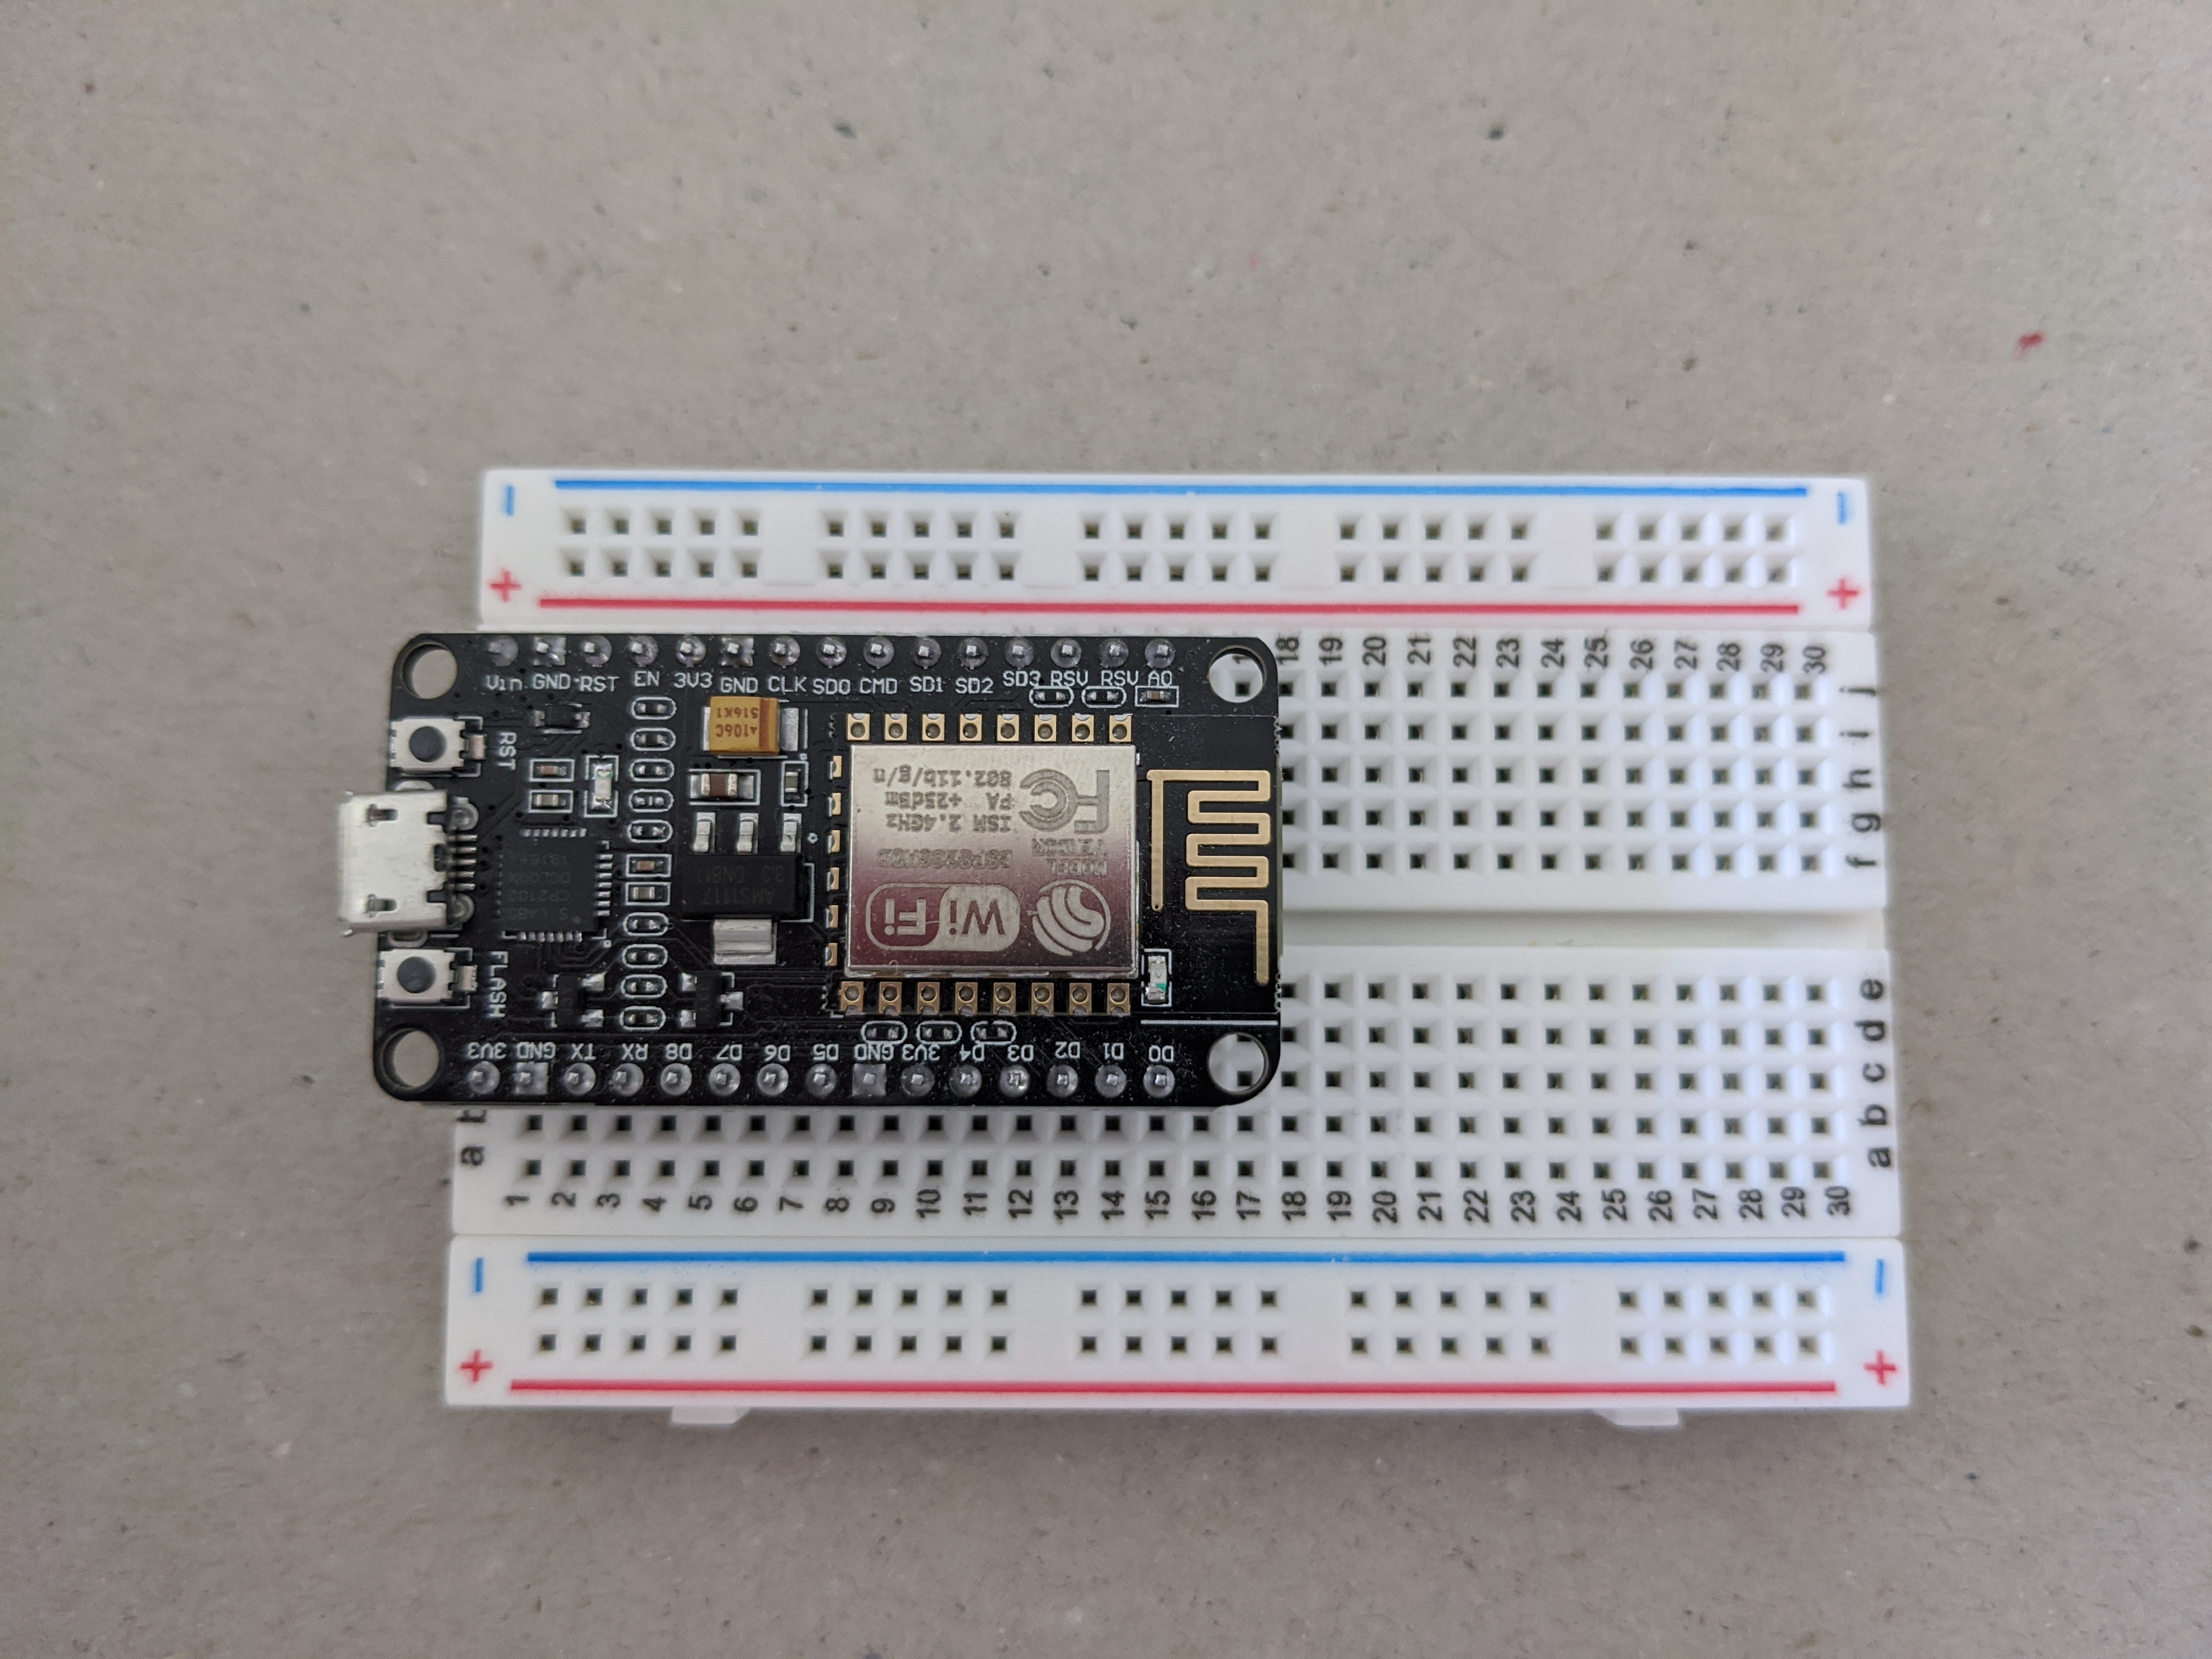
\includegraphics[width=.6\linewidth]{chapter_1/microcontroller_seated_in_breadboard.jpg}
    \caption{So far, so good!}
    \label{fig:microntroller+breadboard}
\end{figure}

\subsubsection{Connect your microcontroller to the positive and negative rails of your breadboard}
% Should we have an overview of components before this? Will the girls know what a 'jumper wire' is? Or the layout of the breadboard?
Using a jumper wire, pin one end of the wire into hole \textbf{A1} of the breadboard and the other end on \textit{any} hole in the column labelled with a \textbf{+} on the side of the breadboard. This column is called the \textbf{positive rail}, and will eventually move power from your microcontroller around the circuit we are building.

Using another jumper wire, pin one end of the wire into hole \textbf{A2} and the other into \textit{any} hole in the column labelled with a \textbf{-} on the side of the breadboard. This column is called the \textbf{negative rail} and, like the positive rail, helps to move power around the circuit we are building.

You should be left with something that looks like this:
\begin{figure}[h!]
    \centering
    \includegraphics[width=.6\linewidth]{chapter_1/positive_and_negative_rails_connected.jpg}
    \caption{I'm absolutely POSITIVE I connected everything correctly!}
    \label{fig:positives_and_negatives}
\end{figure}

\subsubsection{Connect microcontroller to LED}

\subsubsection{Connect resistor between LED and negative power rail}

\subsection{Programming the microcontroller}

\section{Review}
% go over what we have accomplished (maybe go into more detail about the circuit and the pins on the microcontroller?

\section{Possible Extensions}
% ideas to expand this project: Add a second light? write a morse code program?

\end{document}
\chapter{Project 2: Button}
% chapter contents
\chapter{Project 3: LED Party}
% chapter contents
\chapter{Project 4: Sensor}
% chapter contents
\chapter{Project 5: Sound}
% chapter contents

\chapter{Project 6: Chat}
% chapter contents
\chapter{Project 7: Chat}
% chapter contents


\appendix
\chapter{Electronics Essentials}
% chapter contents
\chapter{Python Primer}
% chapter contents

\end{document}
